\documentclass[tikz, border=1mm]{standalone}

\newcommand{\arst}{0.5}

\begin{document}
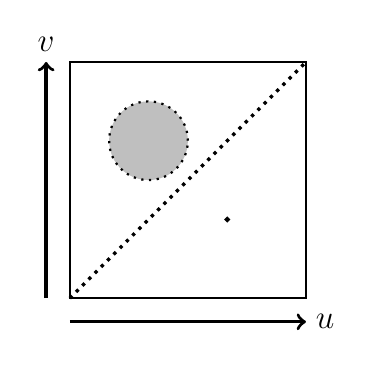
\begin{tikzpicture}[x=1cm, y=1cm, inner sep=0.05in, outer sep=0in]

  % Draw the square
  \draw[thick, black] (0,0) rectangle (3,3);
  % Draw the dotted line from the lower left to the upper right
  \draw[dotted, very thick, black] (0,0) -- (3,3);

  % dot
  \draw[thick, fill=black] (2,1) circle (0.02);

  % dotted circle
  \draw[thick, black, dotted, fill=lightgray] (1,2) circle (0.5);

  \draw[->, very thick] (0, -0.3) -- (3, -0.3) node[anchor=west] {\large $u$};
  \draw[->, very thick] (-0.3, 0) -- (-0.3, 3) node[anchor=south] {\large $v$};
\end{tikzpicture}
\end{document}
